\begin{figure}[!ht]
	\centering
	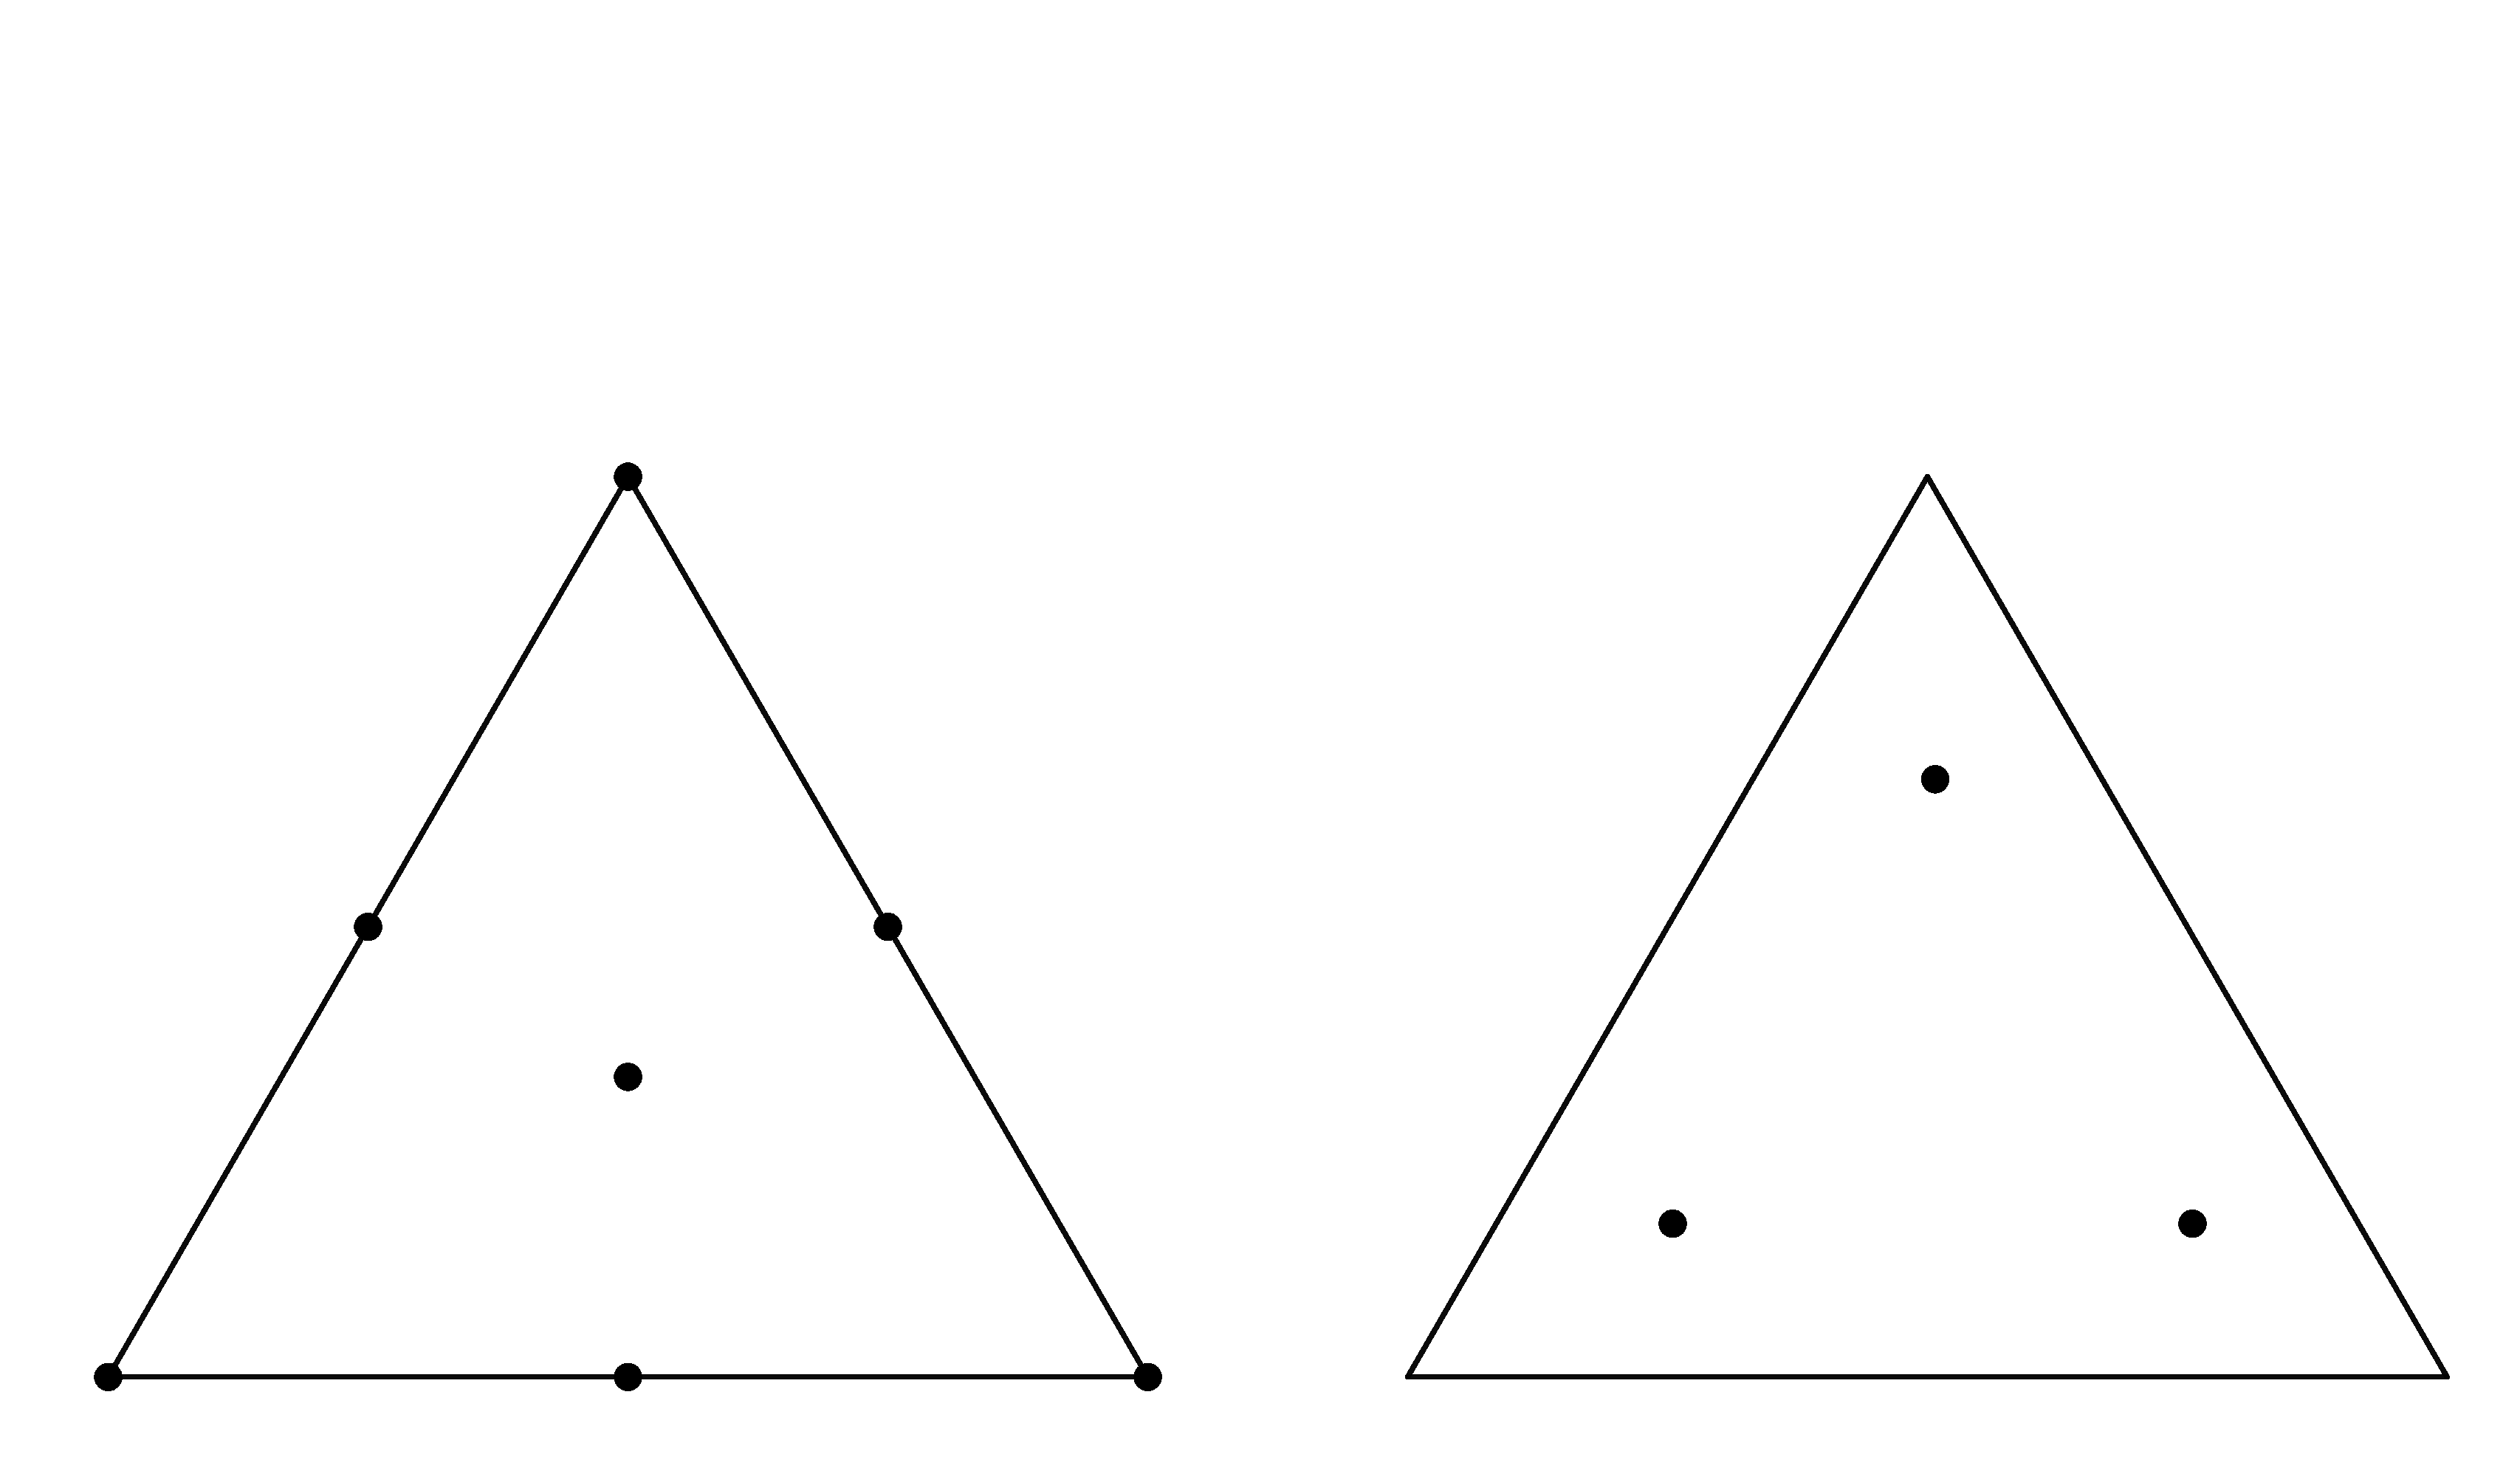
\includegraphics[trim=0cm 8cm 0cm 10cm, clip, width=15cm]{cr.pdf}
	\caption{Crouzeix-Raviart local DOFs for velocity and pressure.}
\end{figure}

Let $\{\Tau_h\}_h$ be a sequence of shape-regular and quasi-uniform meshes. Define $V_h$ and $Q_h$ as follows:

\begin{align}
    V_h &= \left\{ \Vector{v_h} \in \HO_0(\Omega): \Vector{v_h} \vert_T \in \left[ \PK{2}(T) \cup \Span{b_T} \right]^2 ~ \Forall T \in \Tau_h \right\}, \\
    Q_h &= \left\{ q_h \in \LT_0(\Omega): q_h \vert_T \in \PK{1}(T) ~ \Forall T \in \Tau_h \right\},
\end{align}

where $b_T \in \PK{3}(T)$ such that $b_T \vert_{\partial T} = 0$ and $b_T(\nu_T) = 1 ~ \Forall T \in \Tau_h$:

\subsection{Fortin Operator}

Consider the following result.

\begin{lemma}[Fortin] \label{fortin}
    Let $(V, Q)$ be spaces for the Stokes problem for which the continuous \textit{inf-sup} property holds, and let $(V_h, Q_h)$ be the discrete spaces. Let $\fortin: V \rightarrow V_h$ such that for all $\Vector{v} \in V$:
    \begin{enumerate}[i.]
        \item There exists $C \in \R_+$ such that $\lVert \fortin \Vector{v} \rVert_V \leq C \lVert \Vector{v} \rVert_V$,
        \item $\bob{\fortin \Vector{v}}{q_h} = \bob{\Vector{v}}{q_h}$ for all $q_h \in Q_h$,
    \end{enumerate}
    then the discrete \textit{inf-sup} property holds for $(V_h, Q_h)$.
\end{lemma}

Verifying this property for the Crouzeix-Raviart element is necessary to ensure its well-posedness.

\newpage
\noindent Let $\tfortin: V \rightarrow V_h$ such that:

\begin{gather}
    \tfortin \Vector{v} \vert_T = \frac{1}{\theta_T} \left[ \int_T \diver \Vector{v} \begin{pmatrix}
        x - x_T \\
        y - y_T
    \end{pmatrix} \right] \Vector{b_T},
\end{gather}

the Fortin operator $\fortin: V \rightarrow V_h$ for the Crouzeix-Raviart element is defined as follows:

\begin{gather}
    \fortin \Vector{v} = \fortinptpz \Vector{v} + \tfortin \left( \Vector{v} - \fortinptpz \Vector{v}\right),
\end{gather}

where $\fortinptpz$ is the Fortin operator for the $\PK{2}\PK{0}$ element.

$\fortin$ satisfies the hypothesis of the \nameref{fortin} lemma, ensuring the discrete \textit{inf-sup} property for the Crouzeix-Raviart element.

\subsection{Convergence}

The following result can be stated:

\begin{proposition} \label{convergence}
    Let $\{\Tau_h\}_h$ be a sequence of shape-regular and quasi-uniform meshes. Suppose $(\Vector{u}, p)$ is the solution of \eqref{weak_stokes}, and $(\Vector{u_h}, p_h)$ is the solution of \eqref{fem_stokes}. Then there exist $C_1, C_2, C_3 \in \R_+$ such that:

    \begin{gather}
        \lVert \Vector{u} - \Vector{u_h} \rVert_V + \lVert p - p_h \rVert_Q \leq C_1 \inf_{\Vector{v_h} \in V_h} \lVert \Vector{u} - \Vector{v_h} \rVert_V + C_2 \inf_{q_h \in Q_h} \lVert p - q_h \rVert_Q \leq C_3 h^2.
    \end{gather}
\end{proposition}

Quadratic convergence can be expected for the Crouzeix-Raviart element, which will be evaluated in the subsequent section.